%====================================================================================
\section[Ejemplo]{Ejemplos numéricos}
%====================================================================================

\begin{frame}{1. Información simétrica y calidad conocida}
	\begin{center}
		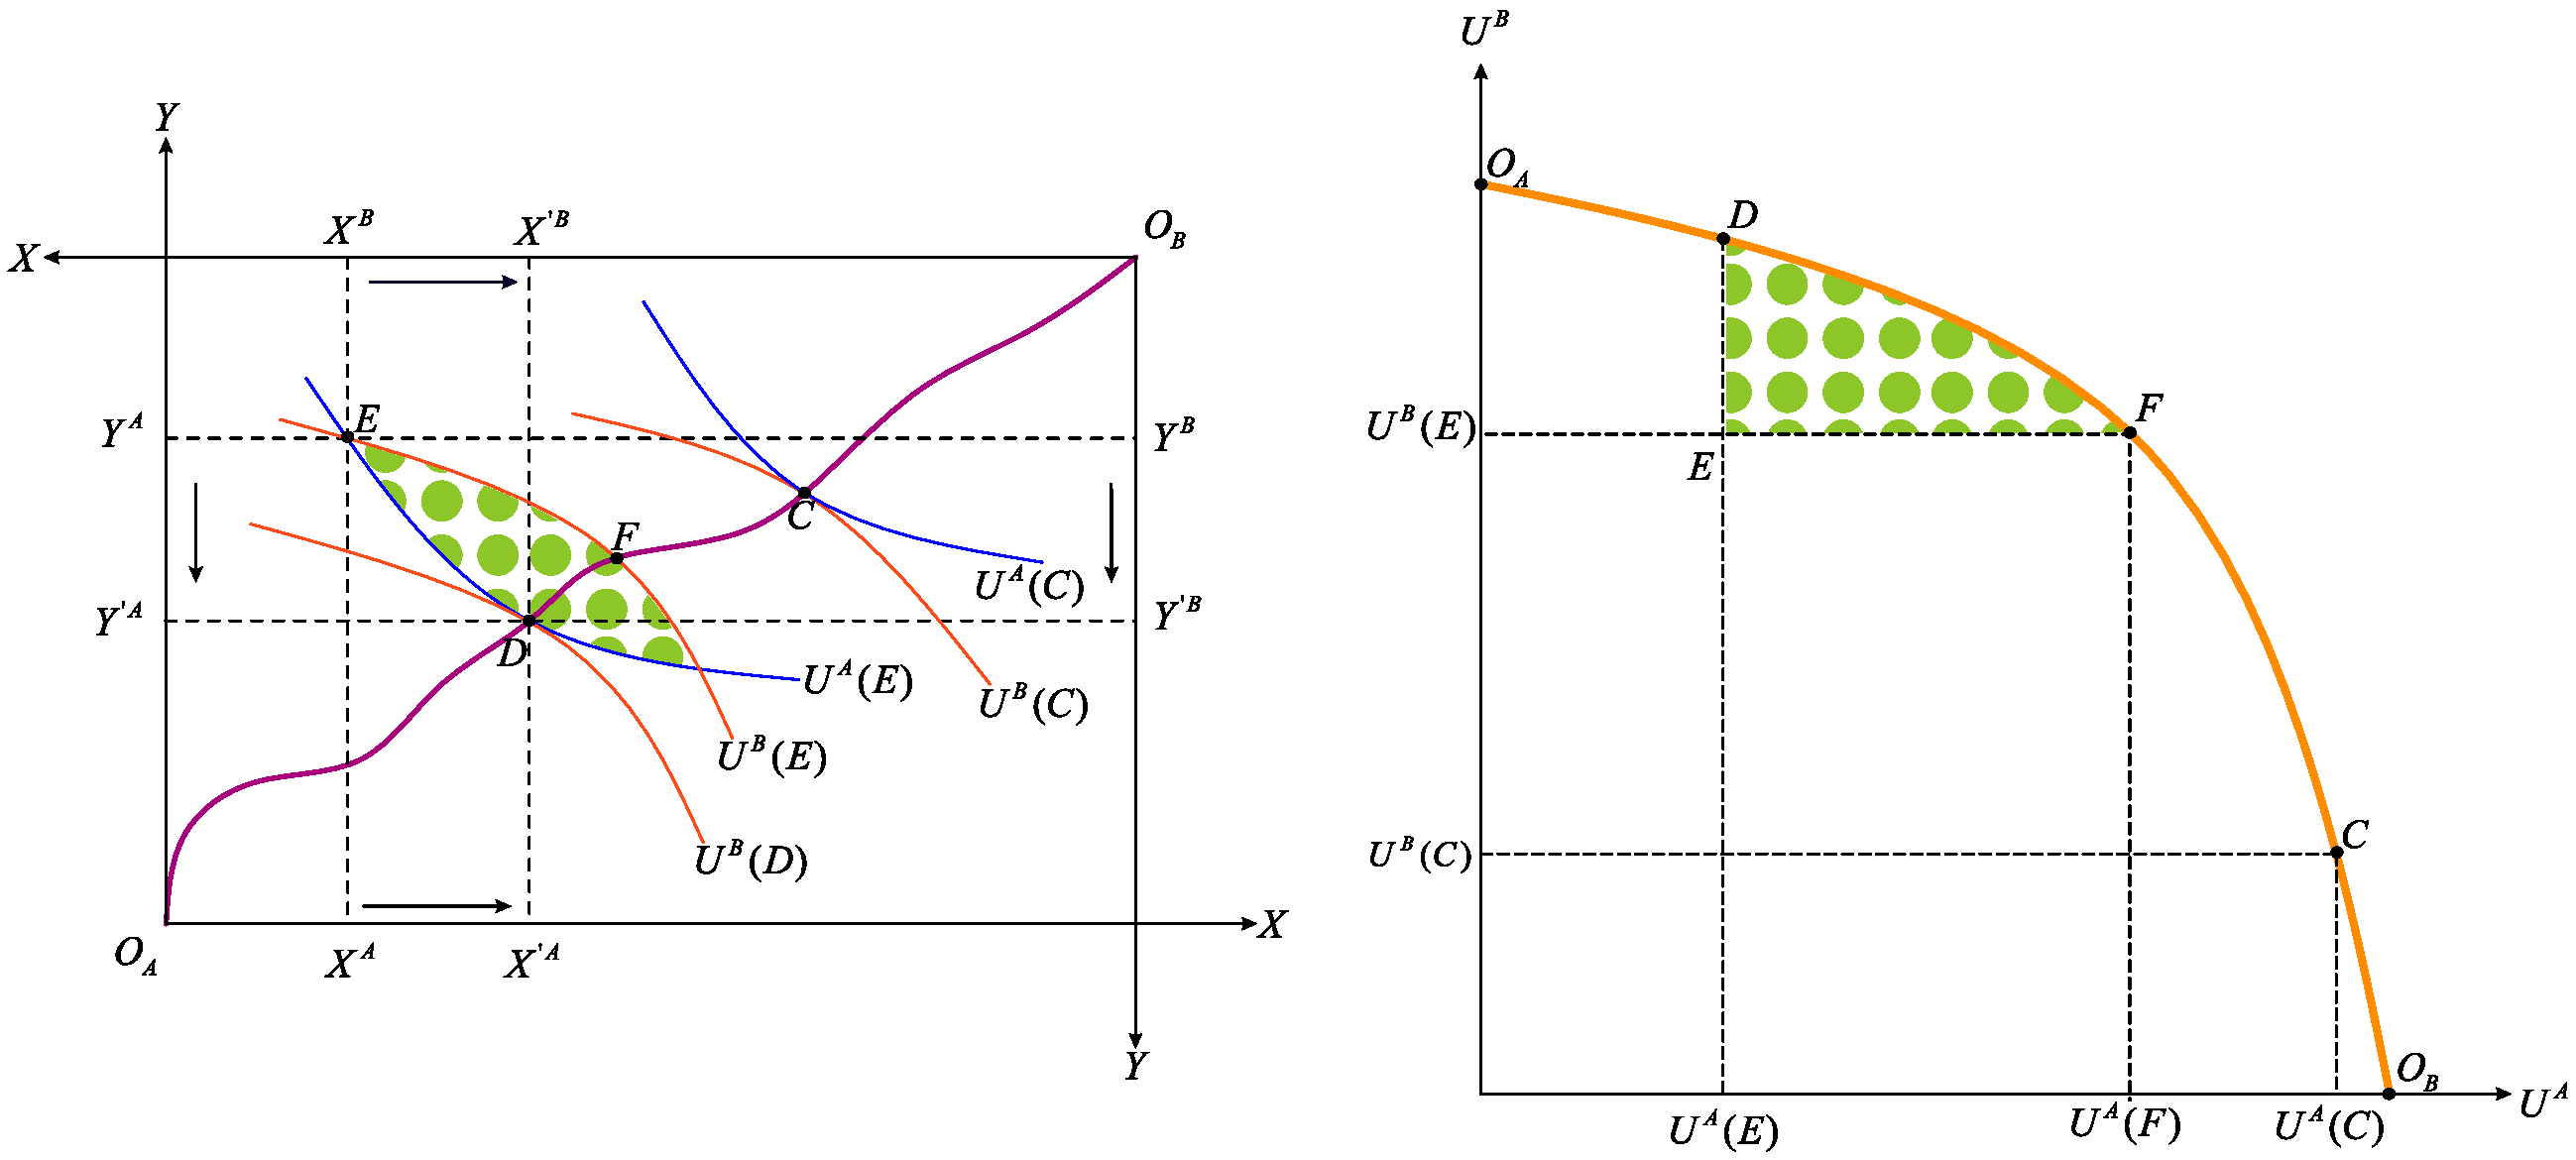
\includegraphics[width = 1\linewidth]{figures/fig_01.png}
	\end{center}
\end{frame}
%------------------------------------------------
\begin{frame}{1. Información simétrica y calidad conocida}
	\begin{center}
		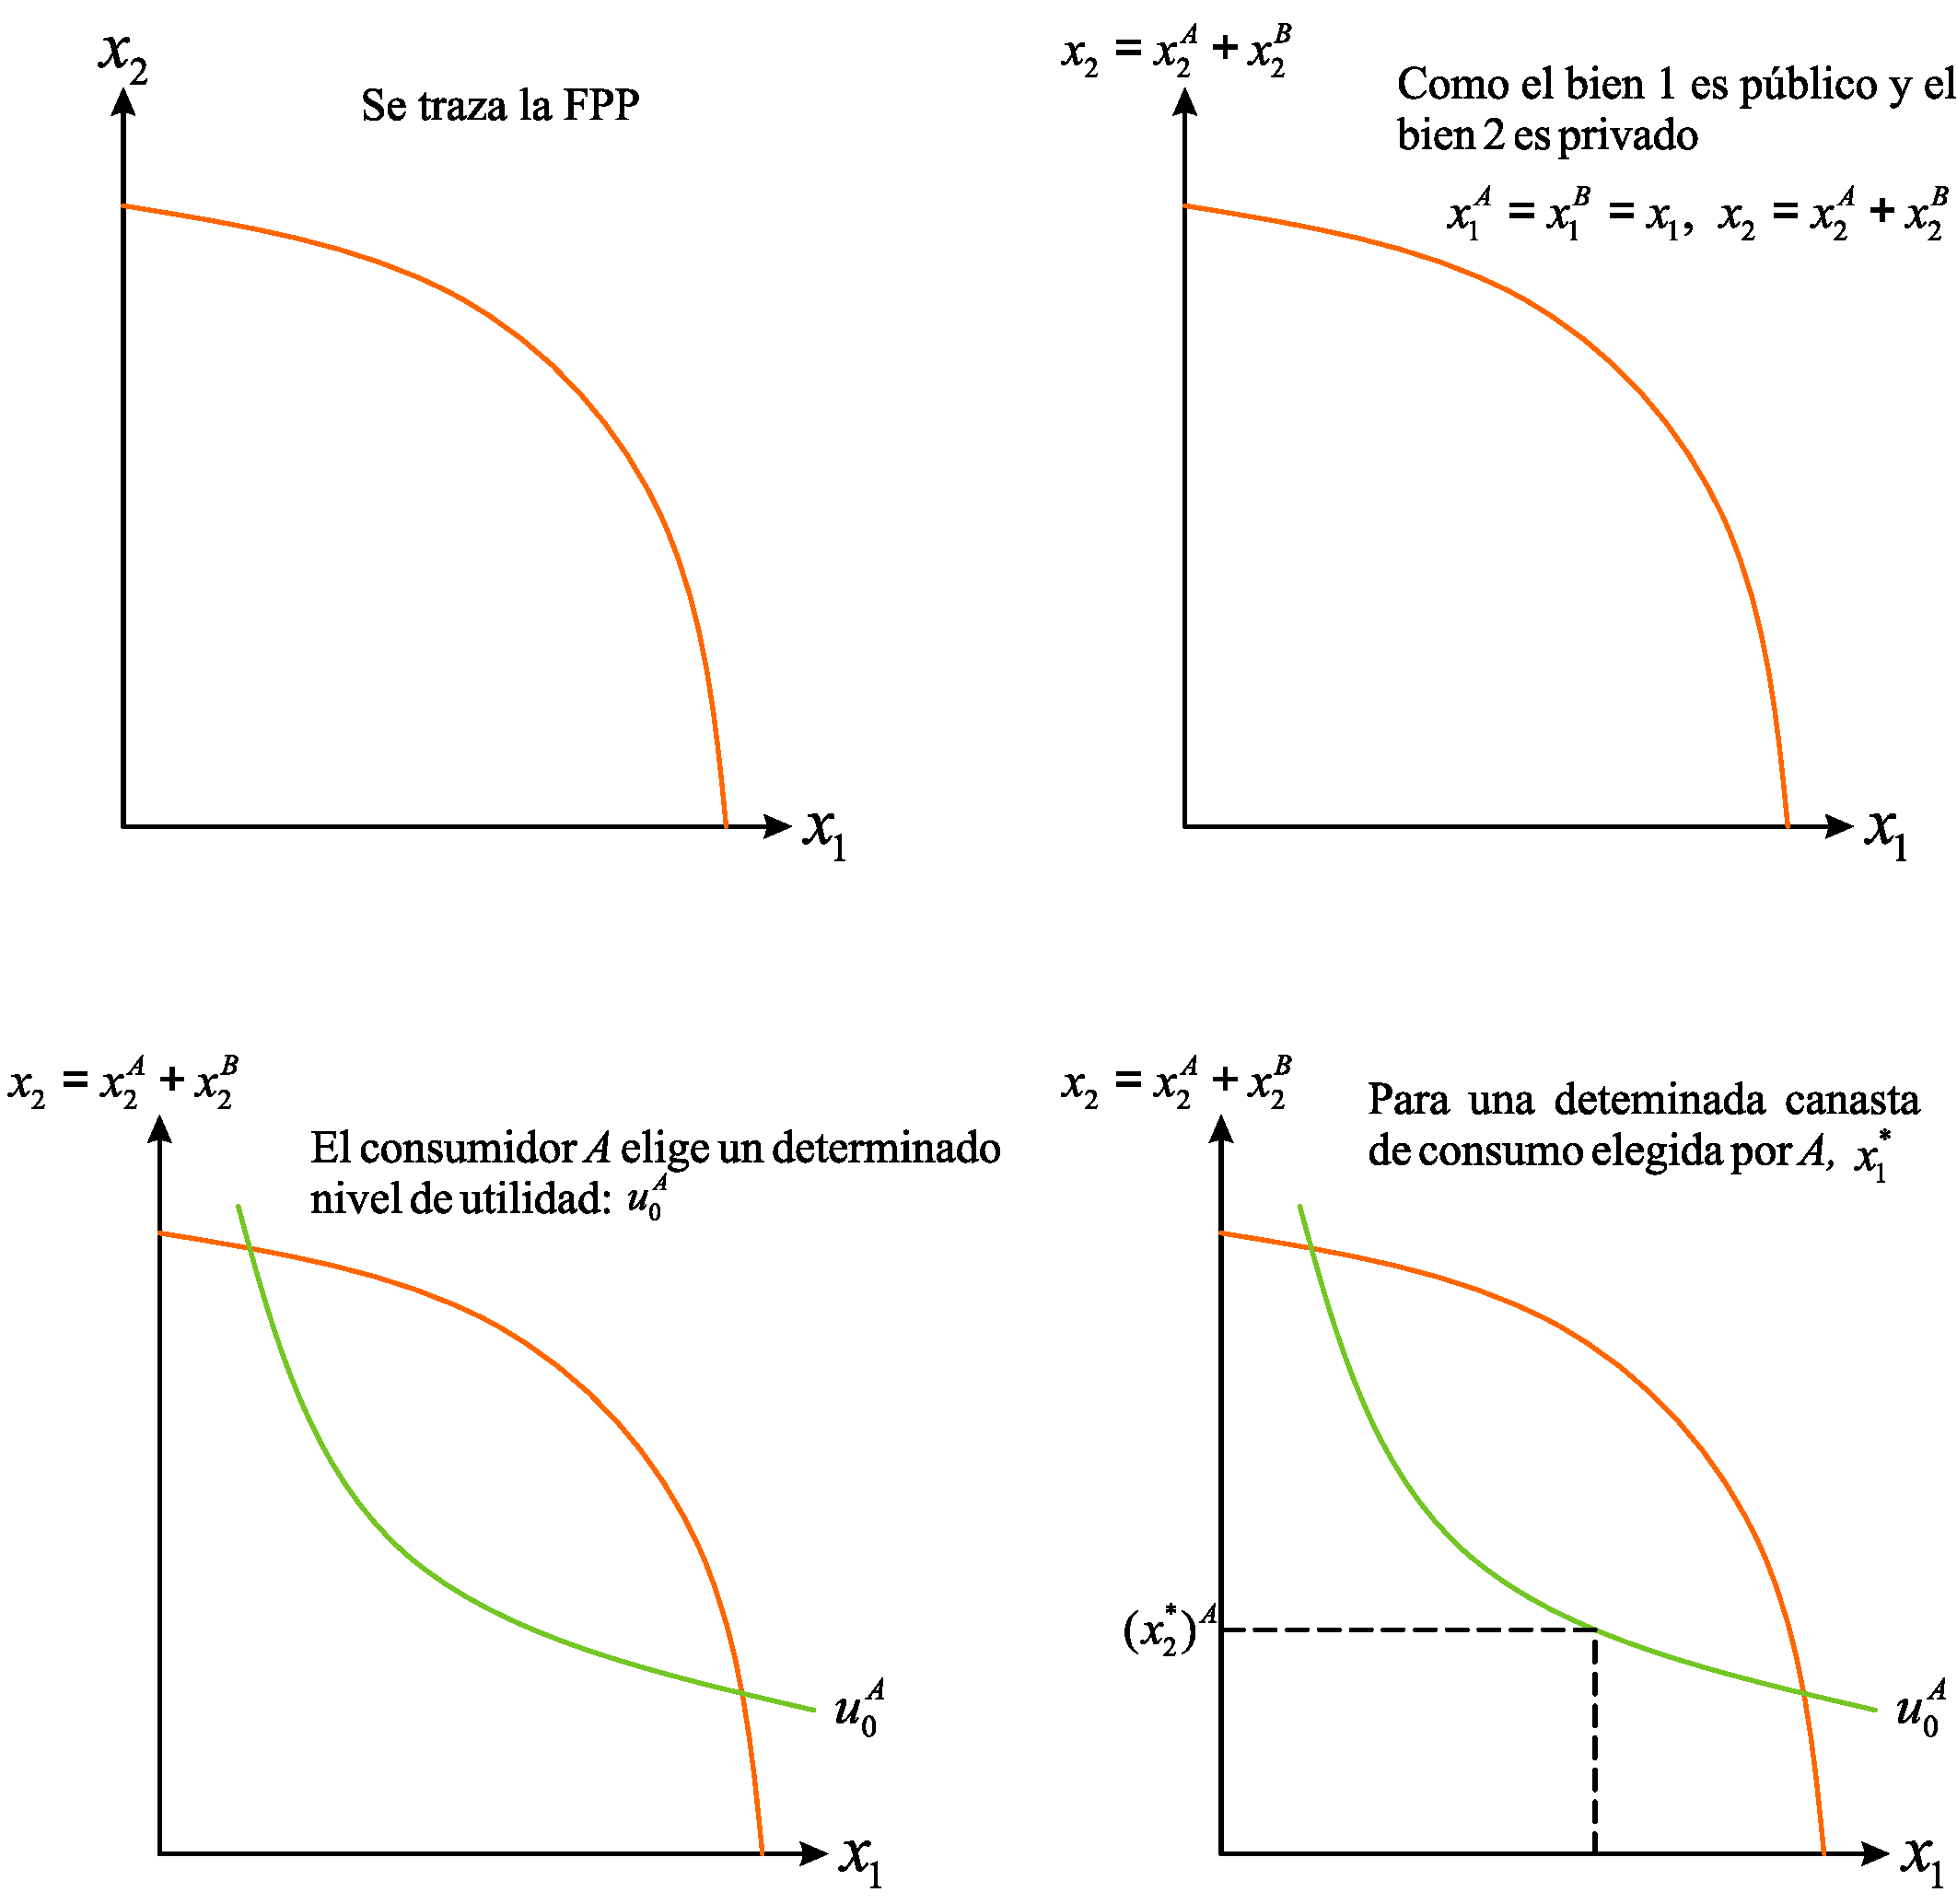
\includegraphics[width = 1\linewidth]{figures/fig_02.png}
	\end{center}
\end{frame}
%------------------------------------------------
\begin{frame}{1. Información simétrica y calidad conocida}
	\begin{center}
		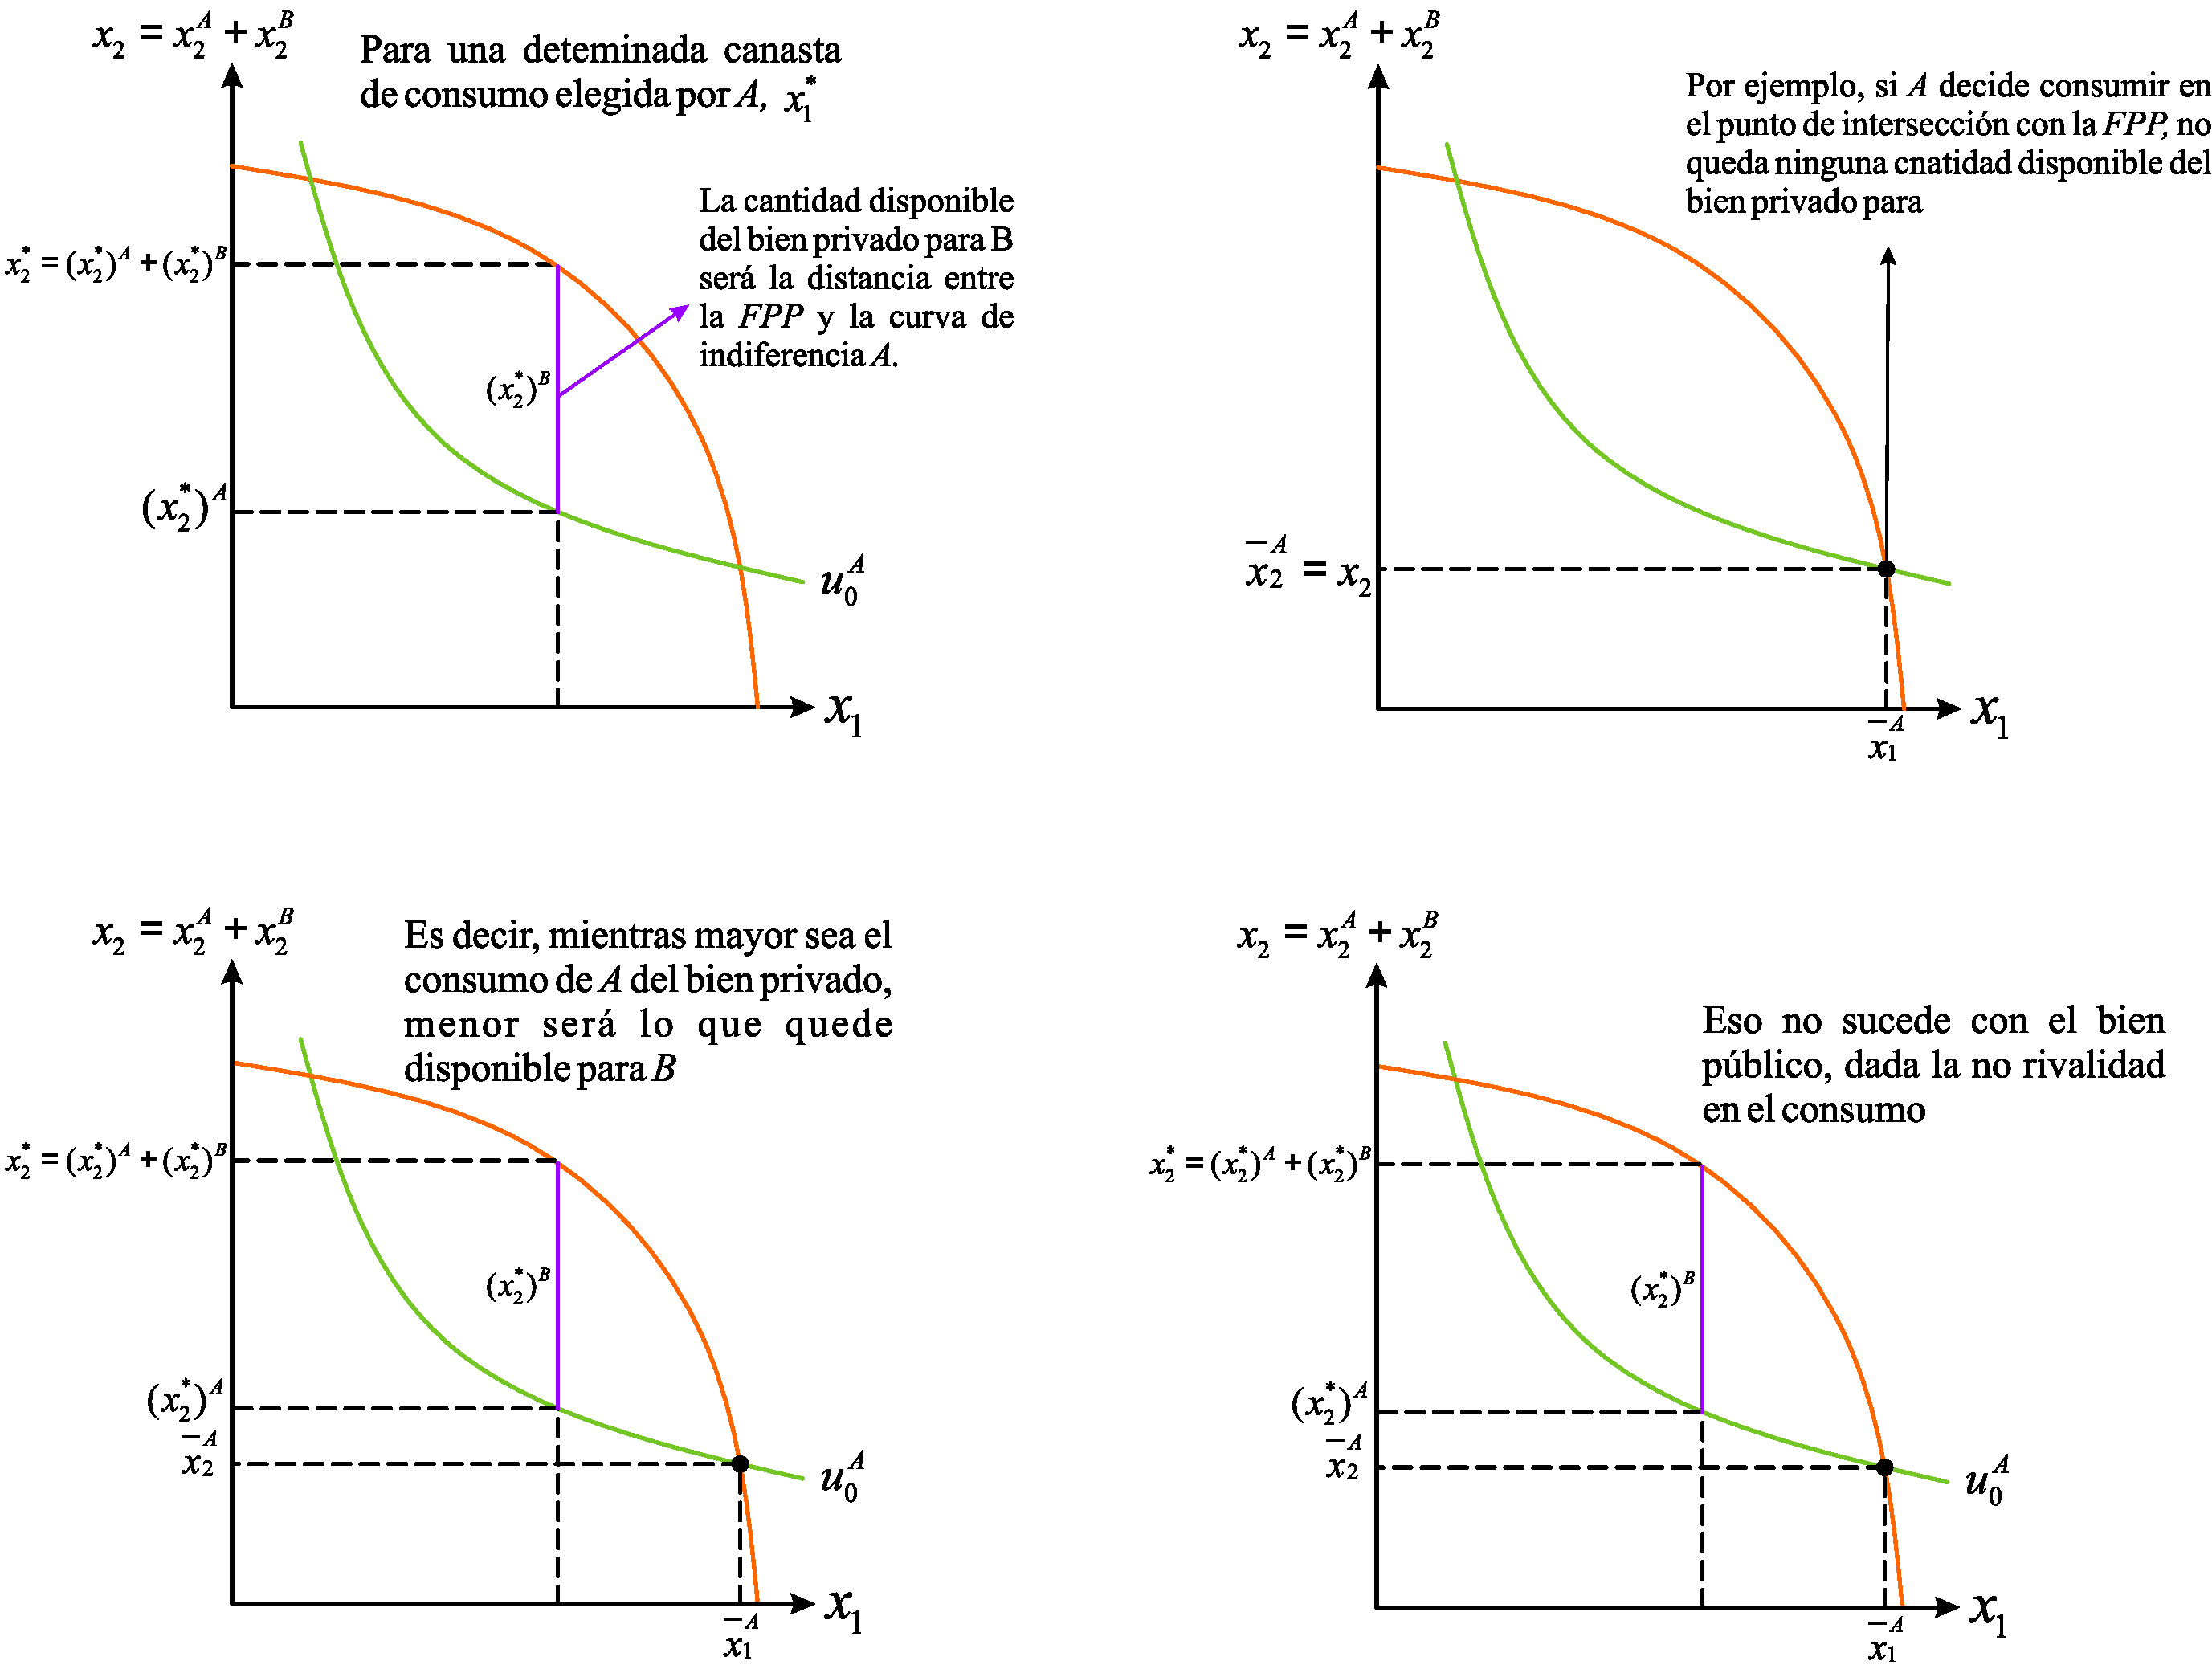
\includegraphics[width = 1\linewidth]{figures/fig_03.png}
	\end{center}
\end{frame}
%------------------------------------------------
\begin{frame}{1. Información simétrica y calidad conocida}
	\begin{center}
		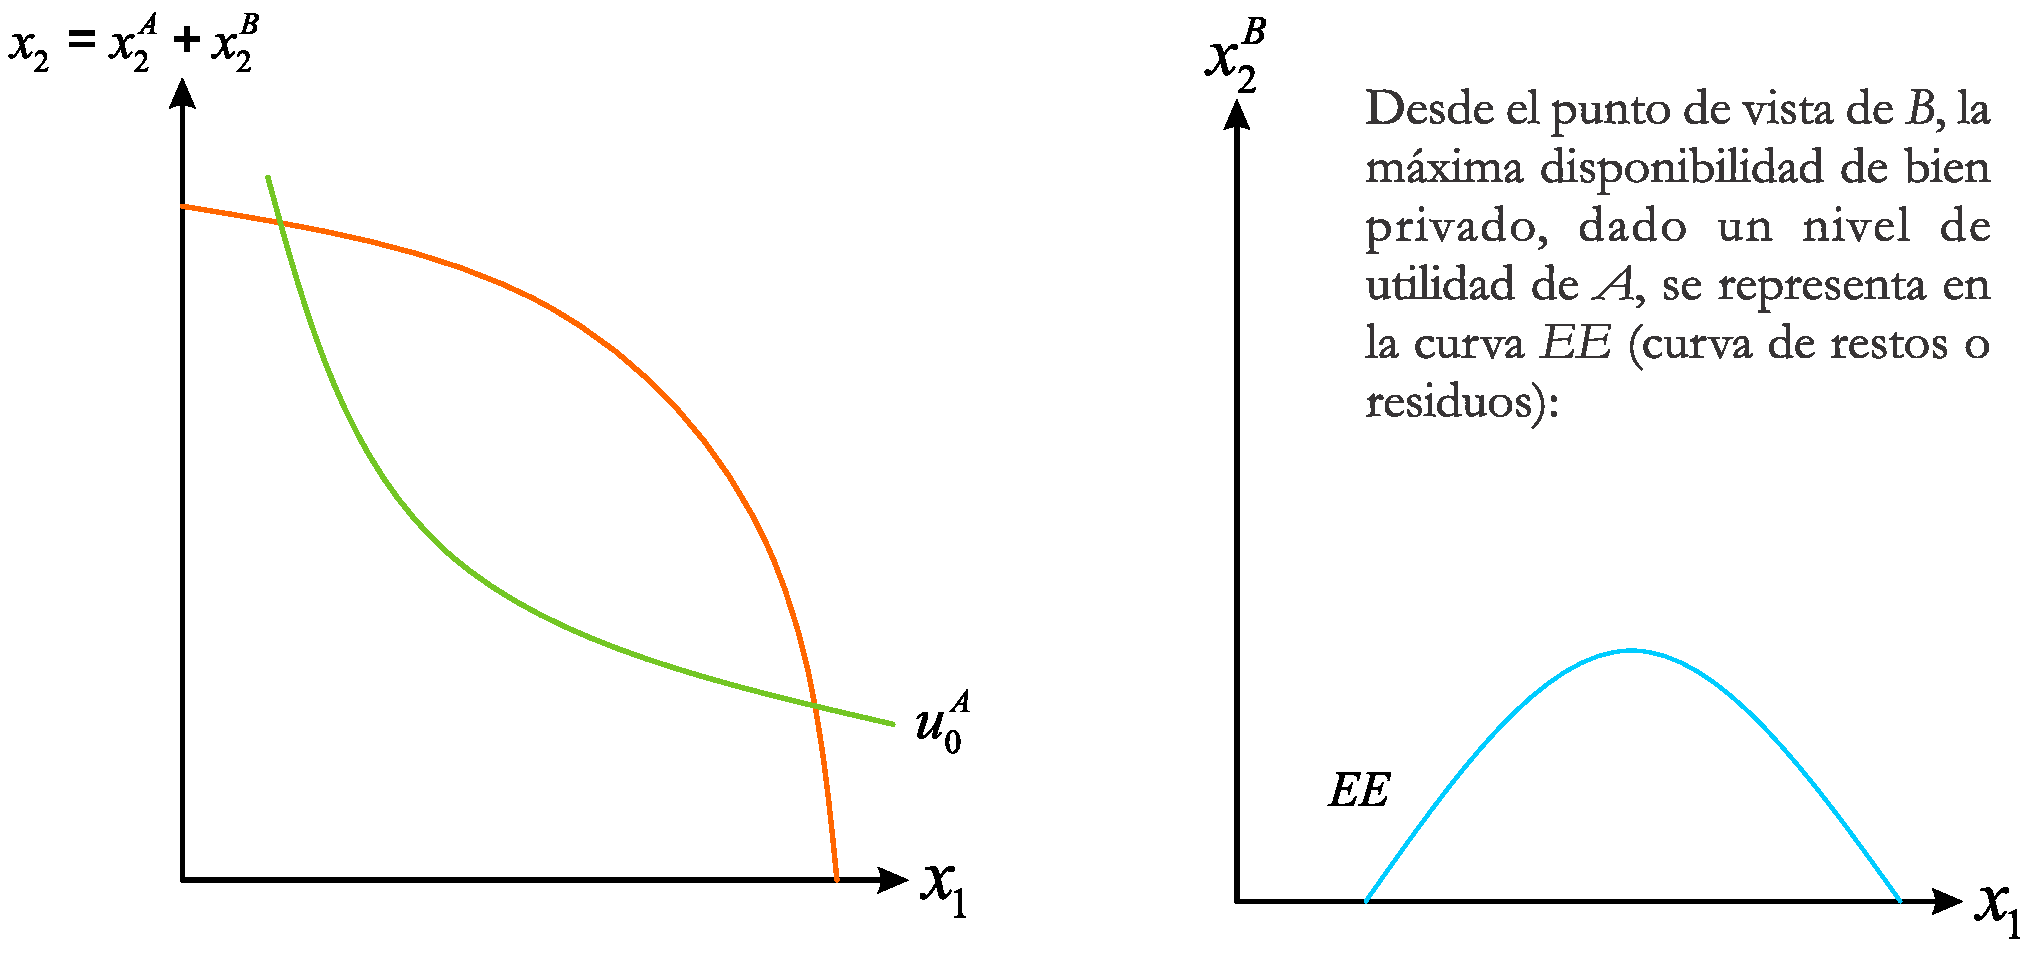
\includegraphics[width = 1\linewidth]{figures/fig_04.png}
	\end{center}
\end{frame}
%------------------------------------------------
\begin{frame}{2. Información simétrica y calidad desconocida}
	\begin{center}
		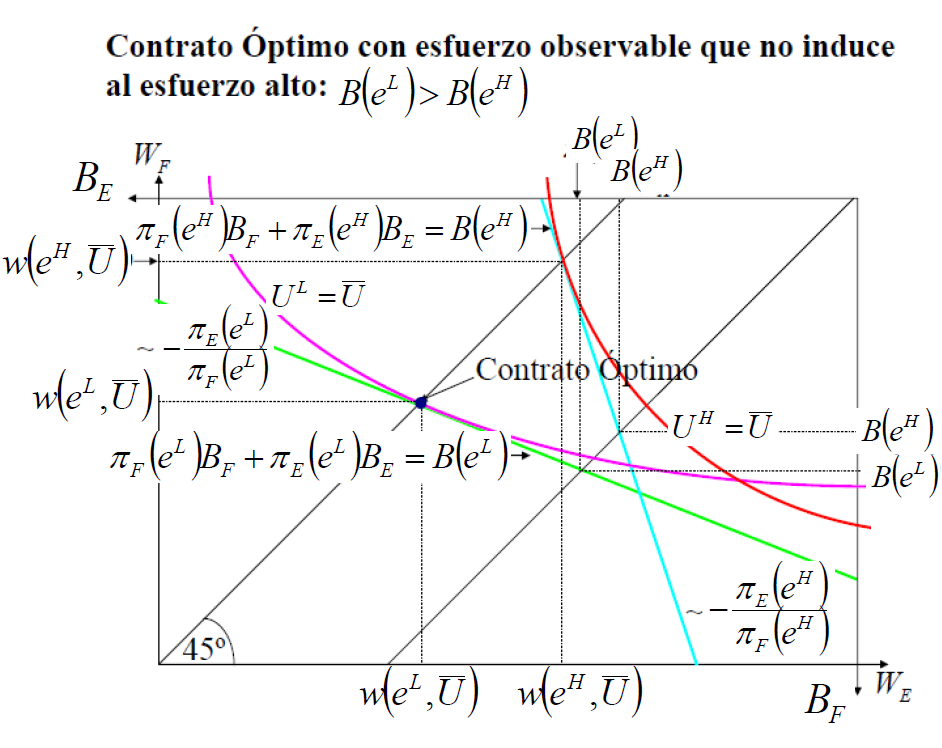
\includegraphics[width = 0.8\linewidth]{figures/fig_05.png}
	\end{center}
\end{frame}
%------------------------------------------------
\begin{frame}{2. Información simétrica y calidad desconocida}
	\begin{center}
		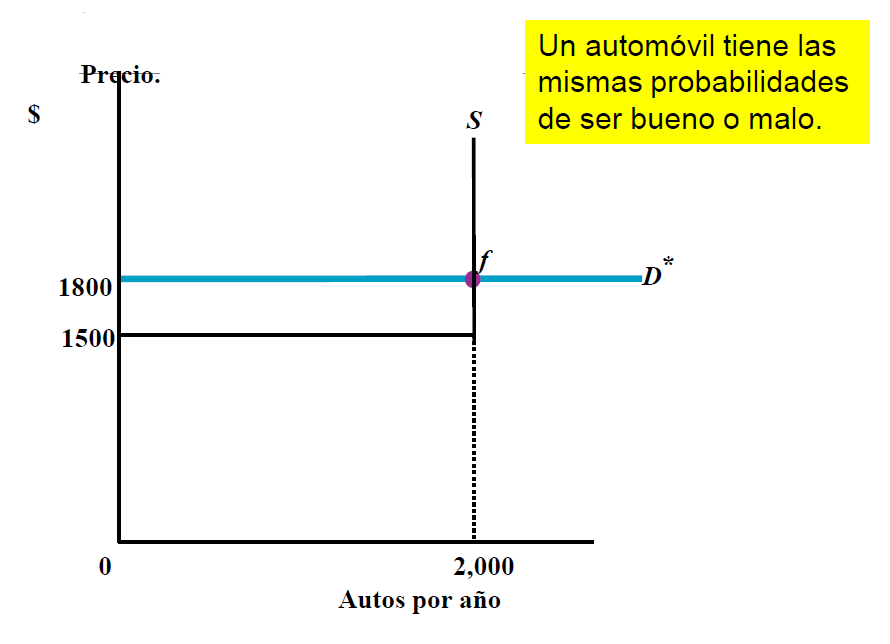
\includegraphics[width = 0.9\linewidth]{figures/fig_06.png}
	\end{center}
\end{frame}
%------------------------------------------------
\begin{frame}{2. Información simétrica y calidad desconocida}
	\begin{center}
		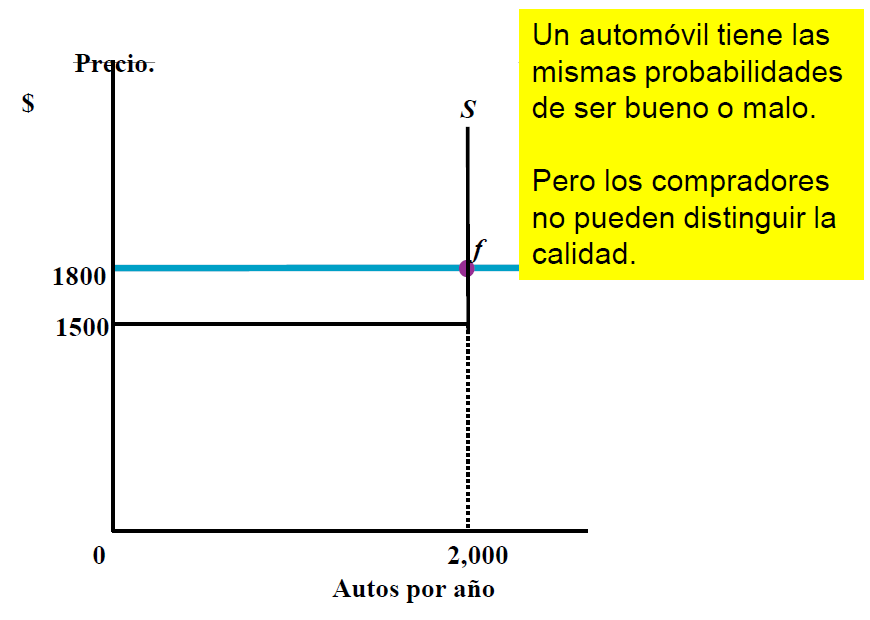
\includegraphics[width = 0.9\linewidth]{figures/fig_07.png}
	\end{center}
\end{frame}
%------------------------------------------------
\begin{frame}{2. Información simétrica y calidad desconocida}
	\begin{center}
		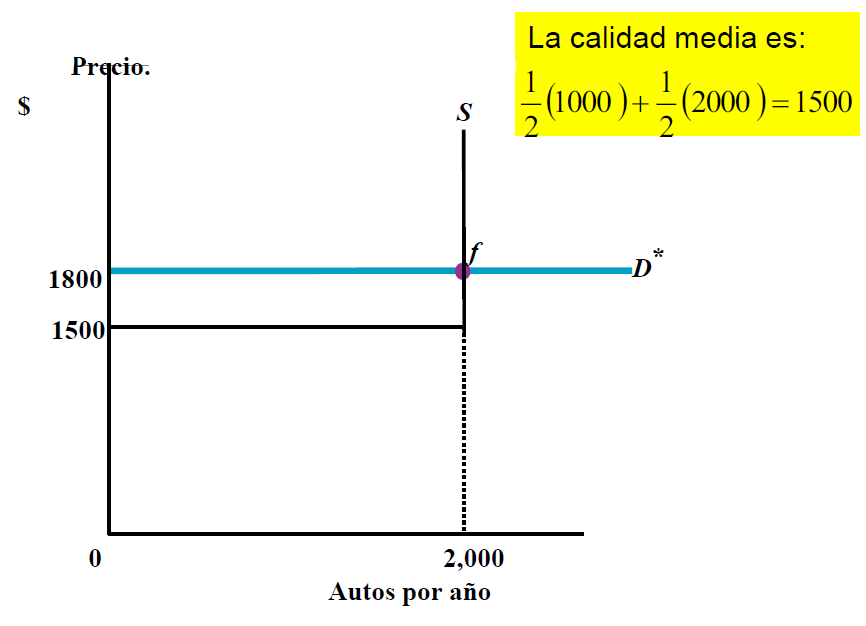
\includegraphics[width = 0.9\linewidth]{figures/fig_08.png}
	\end{center}
\end{frame}
%------------------------------------------------
\begin{frame}{2. Información simétrica y calidad desconocida}
	\begin{center}
		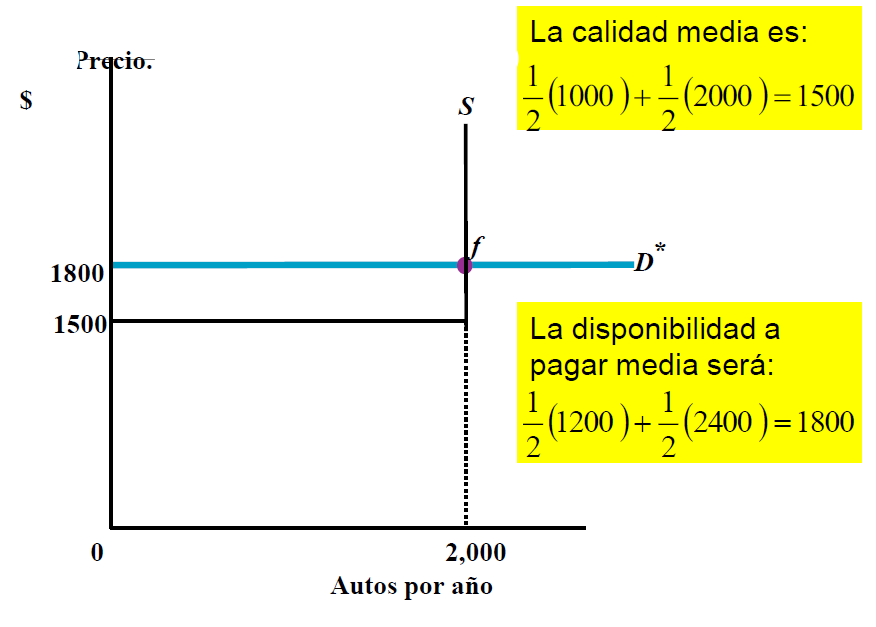
\includegraphics[width = 0.9\linewidth]{figures/fig_10.png}
	\end{center}
\end{frame}
%------------------------------------------------
\begin{frame}{2. Información simétrica y calidad desconocida}
	\begin{center}
		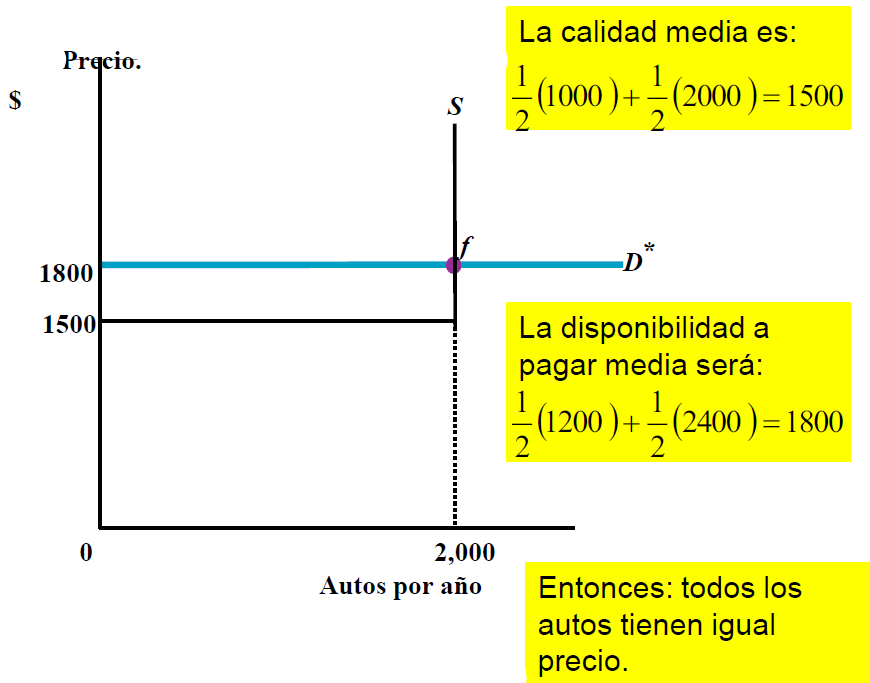
\includegraphics[width = 0.9\linewidth]{figures/fig_11.png}
	\end{center}
\end{frame}
%------------------------------------------------
\begin{frame}{3. Información asimétrica}
	Todos los autos deben venderse al mismo precio, ya que los compradores no pueden distinguir los autos buenos de los malos.\\[0.3cm]
	
	Si el precio es $p$, sólo se venden aquellos autos tales que $\theta < p$.\\[0.3cm]
	
	¿Cuánto es lo máximo que un comprador estaría dispuesto a pagar por
	un auto?\\[0.3cm]
	
	Sean q la fracción de autos buenos y 1 - q la fracción de los autos malos.\\[0.3cm]
	
	El precio máximo que estaría dispuesto a pagar un comprador será
		$$p_m = \$1200(1-q)+\$2400q$$
\end{frame}
%------------------------------------------------
\begin{frame}{3. Información asimétrica}
	\begin{itemize}
		\item Supongamos que $P_m > \$2000$.
			\begin{itemize}
				\item Cada vendedor puede negociar un precio entre $\$2000$ y $P_m$ (sin importar si el carro es malo o bueno).
				\item Todos los vendedores ganan en el mercado.
			\end{itemize}
		\item Supongamos que $P_m < \$2000$.
			\begin{itemize}
				\item Un vendedor de un auto bueno no puede negociar un precio superior a $\$2000$ y saldrá del mercado
				\item Por tanto, todos los compradores conocen que los vendedores restantes sólo tienen carros malos
				\item Los compradores pagarán a lo más $\$1200$ y sólo los autos malos son vendidos
			\end{itemize}
	\end{itemize}
\end{frame}
%------------------------------------------------
\begin{frame}{3. Información asimétrica}
	Por tanto , los autos malos desplazan a los buenos del mercado \\[0.3cm]
	Las ganancias del intercambio se reducen , debido a que los autos buenos no son comercializados\\[0.3cm]
	La presencia de autos malos inflinge un costo externo negativo a los compradores y propietarios de autos buenos\\[0.3cm]
	¿Cuántos autos malos pueden estar en el mercado sin desplazar a los buenos?\\[0.3cm]
	Los compradores pagarán $\$2000$ por un auto sólo si
		$$ p_m = \$1200(1-q)+\$2400q \geq \$2000 $$
	Por tanto, si más de un tercio de los autos son malos, sólo se venderán autos malos.
		$$ q \geq \frac{2}{3} $$
	De allí el nombre: selección adversa
\end{frame}
%------------------------------------------------
\begin{frame}{3. Información asimétrica}
	¿Qué sucede si hay más de dos tipos de autos?\\[0.3cm]
	Supongamos que
		\begin{itemize}
			\item la calidad de los autos está distribuida uniformemente entre $\$1000$ y $\$2000$
			\item Cualquier auto que un vendedor valorice en $\$x$ es valorado por un comprador en $\$(x+300)$.
		\end{itemize}
	¿Cuáles autos serán transados?
\end{frame}
%------------------------------------------------
\begin{frame}{3. Información asimétrica}
	\begin{center}
		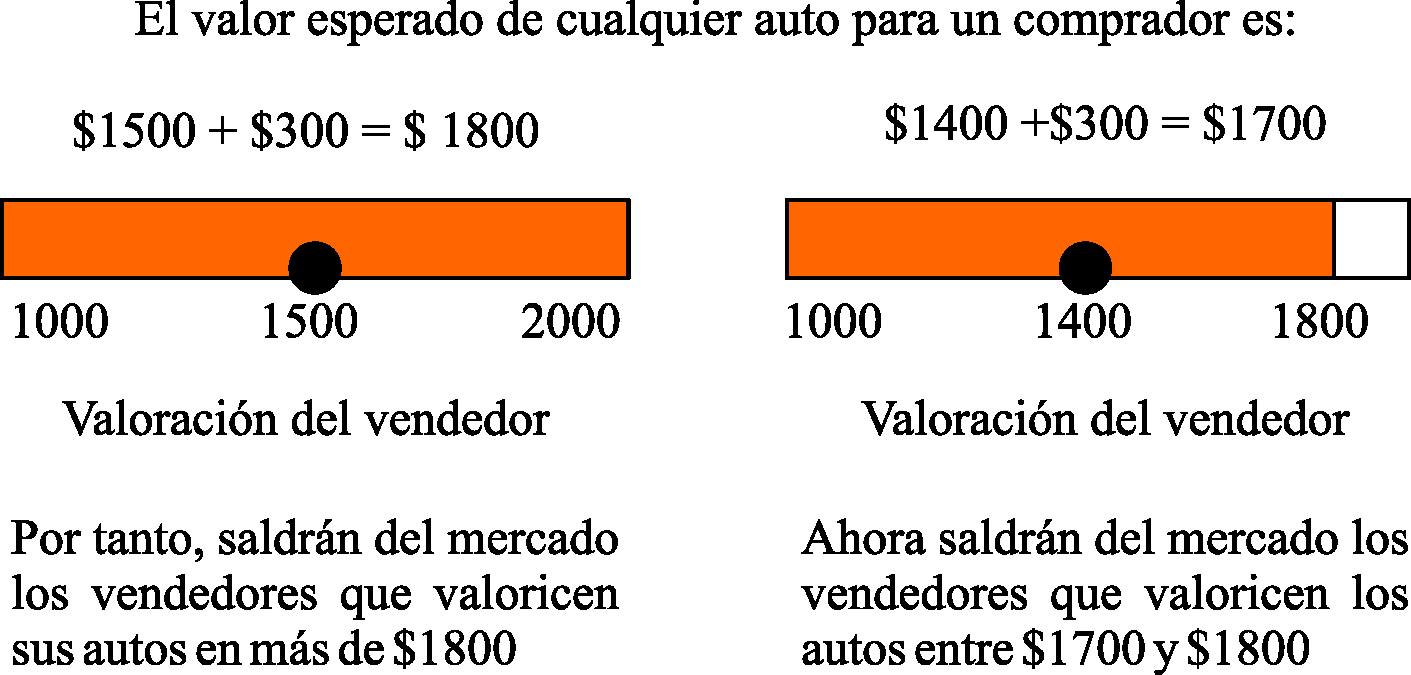
\includegraphics[width = 1\linewidth]{figures/select.pdf}
	\end{center}
\end{frame}
%------------------------------------------------
\begin{frame}{3. Información asimétrica}
	¿Donde termina este ``desenredo'' del mercado?\\[0.3cm]
	Sea $v_H$ la más alta valoración del vendedor de cualquier auto remanente en el mercado.\\[0.3cm]
	El valor esperado del vendedor de un auto es
		$$\frac{1}{2}\times 1000 + \frac{1}{2}\times v_H$$
	Por tanto un comprador pagará a lo más
		$$\frac{1}{2}\times 1000 + \frac{1}{2}\times v_H + 300$$
	Este debe ser el precio aceptado por el vendedor del auto de mayor valor en el mercado; es decir:
		$$\frac{1}{2}\times 1000 + \frac{1}{2}\times v_H + 300 = v_H \longrightarrow v_H = \$1600$$
	La selección adversa elimina los autos valorados por los vendedores más de $\$1600$.
\end{frame}